\documentclass{article}
\usepackage{preamble}

\title{Unit 9: The Earth}
\author{Astronomy\footnote{Access for free at \href{\openstax}{\openstax}} \hspace{0.1ex} at Cypress Springs High School}
\date{Updated on \today}

\numberwithin{equation}{section}
\setcounter{section}{9}
\numberwithin{figure}{section}

\usepackage{fancyhdr}
\pagestyle{fancy}
\renewcommand{\headrulewidth}{0pt}
\renewcommand{\headruleskip}{0mm}
\fancyfoot[C]{Access for free at \href{\openstax}{\openstax} \hfill \thepage}
\fancyhead{}

\makenoidxglossaries

\newglossaryentry{basalt}{
    name=basalt,
    description={igneous rock produced by the cooling of lava; makes up most of Earth's oceanic crust and is found on other planets that have experienced extensive volcanic activity}
}

\newglossaryentry{core}{
    name=core,
    description={the central part of the planet; consists of higher density material}
}

\newglossaryentry{magnetosphere}{
    name=magnetosphere,
    description={the region around a planet in which its intrinsic magnetic field dominates the interplanetary field carried by the solar wind; hence, the region within which charged particles can be trapped by the planetary magnetic field}
}

\newglossaryentry{crust}{
    name=crust,
    description={the outer layer of a terrestrial planet}
}

\newglossaryentry{granite}{
    name=granite,
    description={a type of igneous silicate rock that makes up most of Earth’s continental crust}
}

\newglossaryentry{mantle}{
    name=mantle,
    description={the largest part of Earth's interior; lies between the crust and the core}
}

\newglossaryentry{volcano}{
    name=volcano,
    description={a place where material from a planet's mantle erupts on its surface}
}

\begin{document}

\maketitle

\subsection{Properties of Earth} \label{kdMLi7}

\begin{minipage}{0.55\textwidth}
    Earth is a medium-size planet with a diameter of approximately \SI{12760}{} kilometers. As one of the inner or terrestrial planets, it is composed primarily of heavy elements such as iron, silicon, and oxygen---very different from the composition of the Sun and stars, which are dominated by the light elements hydrogen and helium. Earth's orbit is nearly circular, and Earth is warm enough to support liquid water on its surface. It is the only planet in our solar system that is neither too hot nor too cold, but ``just right'' for the development of life as we know it.
\end{minipage}%
\hspace{5mm}
\begin{minipage}{0.35\textwidth}
\centering
    %\includegraphics[width=8cm]{NASA_Earth.jpeg}
    \begin{tikzpicture}
    \clip (0,0) circle (2.75cm);
    \node at (-0.02,0.08) 
        {\includegraphics[width=6cm,trim={9cm 9cm 9cm 9cm}, clip]{Figures/NASA_Earth.jpeg}};
    %\draw[thick,red] (0,0) circle (2.8cm); % USEFUL FOR MEASURING CLIP
    \end{tikzpicture}
    \captionof*{figure}{\scriptsize Credit: modification of work by NASA}
\end{minipage}

\cyanhrule
\vspace{-1ex}


\subsection*{\ref{kdMLi7} Exercises}

\setlength{\columnsep}{1cm}

% \begin{multicols}{2}

\begin{exercise} \label{uqgC3z}
    Go to \href{https://earth.google.com/}{https://earth.google.com/} (Google Earth). Do NOT adjust any settings. Zoom in on Earth and locate the United States. On the left-hand menu bar, click the ruler icon, which is the bottom-most icon. With this distance tool, you choose multiple points on Earth and it calculates the distance between the points. Chose two coastal locations in the United States, and answer the following questions: Approximately how long is the United States? We'll call this value 1 US length. (Note: You're answer does not have to be exact, as this exercise is simply an estimate.)
\end{exercise}

\begin{exercise}
    Find Texas in \href{https://earth.google.com/}{Google Earth}. Approximately how long is Texas? We'll call this 1 Texas length.
\end{exercise}

\begin{exercise} \label{VbC5xi}
Measure the Earth's circumference, using the following steps: Go to \href{https://earth.google.com/}{Google Earth}. Do NOT adjust any settings. Locate Ecuador and find its capital, Quito. Click the distance tool (the bottom-most icon on the left-hand menu bar). Let's calculate the distance from Quito in an eastern trip around the whole world. The overall path will look like a great circle wrapping around the planet near the equator. This path is best created in steps, using the following locations as points in your distance measurement:

\begin{enumerate}
\setlength\itemsep{-0.5ex}
    \item Quito, Ecuador
    \item Nairobi, Kenya
    \item Singapore, Singapore
    \item Nauru
    \item Isla Santiago, Galapagos Islands
    \item Quito, Ecuador
\end{enumerate}

Since these locations are near the equator, you are effectively approximating Earth's circumference.
\end{exercise}


\begin{exercise}
Consider a circle of radius $r$:

\begin{center}
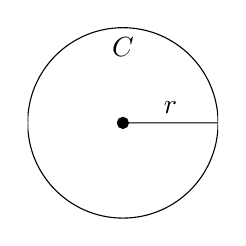
\begin{tikzpicture}
\begin{axis}[width=4cm,height=4cm,
    xmin=-1,xmax=1,ymin=-1,ymax=1,
    axis line style={draw=none},
    ticks=none,
]
\draw (0,0) circle (1);
\draw[fill=black] (0,0) circle (2pt) -- (1,0);
\node[above] at (0.5,0) {$r$};
\node[below] at (0,1) {$C$};

\end{axis}
\end{tikzpicture}
\end{center}

Its circumference (or perimeter) is given by the equation

\begin{equation*}
    C = 2\pi r
\end{equation*}

While Earth is not a circle but a sphere, the same circumference equation applies to the radius of a sphere. Use the equation above and your answer to Exercise \ref{VbC5xi} to calculate Earth's radius.

\end{exercise}


\begin{exercise}
    What is Earth's diameter? (\textit{Hint}: Diameter is two times the radius.)
\end{exercise}

\begin{exercise} 
    How many US-lengths would fit between the crust and core? (\textit{Hint}: See your answer to Exercise \ref{uqgC3z})
\end{exercise}

\begin{exercise}
    How many Texas-lengths would fit between the crust and core?
\end{exercise}

\begin{exercise}
    How many copies of the United States placed side-by-side around the Earth would fit along Earth's equator?
\end{exercise}

\begin{exercise}
    How many Texas-lengths is Earth's equator?
\end{exercise}

\begin{exercise} \label{BKbf6Y}
    Complete the table below. (\textit{Hint}: Go to Chapter 8 of \href{https://openstax.org/books/astronomy-2e/pages/1-1-the-nature-of-astronomy}{OpenStax Astronomy 2e}).

\begin{center}
\begin{tabular}{|m{5cm}|m{5cm}|}
    \hline
    \textbf{Property} & \textbf{Measurement}\\
    \hline
    Semimajor axis &  \\
    \hline
    Period &  \\
    \hline
    Mass &  \\
    \hline
    Diameter &  \\
    \hline
    Radius & \\
    \hline
    Rotational Period & \\
    \hline
    Escape Velocity & \\
    \hline
    Surface Area & \\
    \hline
    Density & \\
    \hline
    Atmospheric Pressure & \\
    \hline
\end{tabular}
\end{center}
\end{exercise}

\clearpage

\subsection{Earth's Interior} \label{uEEpoG}

The interior of a planet---even our own Earth---is difficult to study, and its composition and structure must be determined indirectly. Our only direct experience is with the outermost skin of Earth's crust, a layer no more than a few kilometers deep. It is important to remember that, in many ways, we know less about our own planet 5 kilometers beneath our feet than we do about the surfaces of Venus and Mars.
\vspace{1em}

\begin{minipage}{0.45\textwidth}
    The top layer is the \gls{crust}, the part of Earth we know best (Figure 8.4). Oceanic crust covers 55\% of Earth's surface and lies mostly submerged under the oceans. It is typically about 6 kilometers (4 miles) thick and is composed of volcanic rocks called \gls{basalt}. Produced by the cooling of volcanic lava, basalts are made primarily of the elements silicon, oxygen, iron, aluminum, and magnesium. The continental crust covers 45\% of the surface, some of which is also beneath the oceans. The continental crust is 20 to 70 kilometers (12 to 43 miles) thick and is composed predominantly of a different volcanic class of silicates (rocks made of silicon and oxygen) called \gls{granite}. These crustal rocks, both oceanic and continental, typically have densities of about \SI{3}{g/cm^3}. (For comparison, the density of water is \SI{1}{g/cm^3}.) The crust is the easiest layer for geologists to study, but it makes up only about 0.3\% of the total mass of Earth.
\end{minipage}%
\hspace{5mm}
\begin{minipage}{0.45\textwidth}
    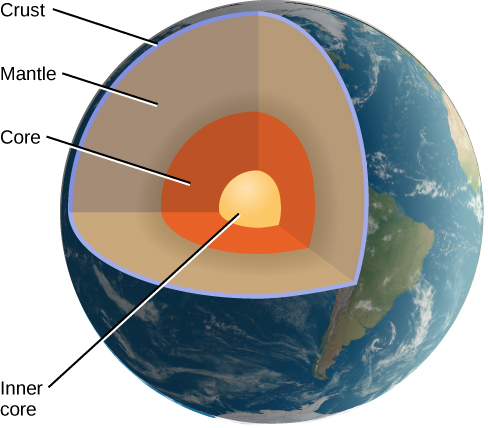
\includegraphics[width=8cm]{Figure8.3.jpg}
\end{minipage}

\vspace{1em}

The largest part of the solid Earth, called the \gls{mantle}, stretches from the base of the crust downward to a depth of 2900 kilometers (1800 miles). The mantle is more or less solid, but at the temperatures and pressures found there, mantle rock can deform and flow slowly. The density in the mantle increases downward from about \SI{3.5}{g/cm^3} to more than \SI{5}{g/cm^3} as a result of the compression produced by the weight of overlying material. Samples of upper mantle material are occasionally ejected from \gls{volcano}es, permitting a detailed analysis of its chemistry.

\vspace{1em}

Beginning at a depth of 2900 kilometers (1800 miles), we encounter the dense metallic \gls{core} of Earth. With a diameter of 7000 kilometers (4350 miles), our core is substantially larger than the entire planet Mercury. The outer core is liquid, but the innermost part of the core (about 1500 miles in diameter) is probably solid. In addition to iron, the core probably also contains substantial quantities of nickel and sulfur, all compressed to a very high density.

\vspace{1em}

The separation of Earth into layers of different densities is an example of differentiation, the process of sorting the major components of a planet by density. The fact that Earth is differentiated suggests that it was once warm enough for its interior to melt, permitting the heavier metals to sink to the center and form the dense core. Evidence for differentiation comes from comparing the planet's bulk density (\SI{5.5}{g/cm^3}) with the surface materials (\SI{3}{g/cm^3}) to suggest that denser material must be buried in the core.

\begin{center}
    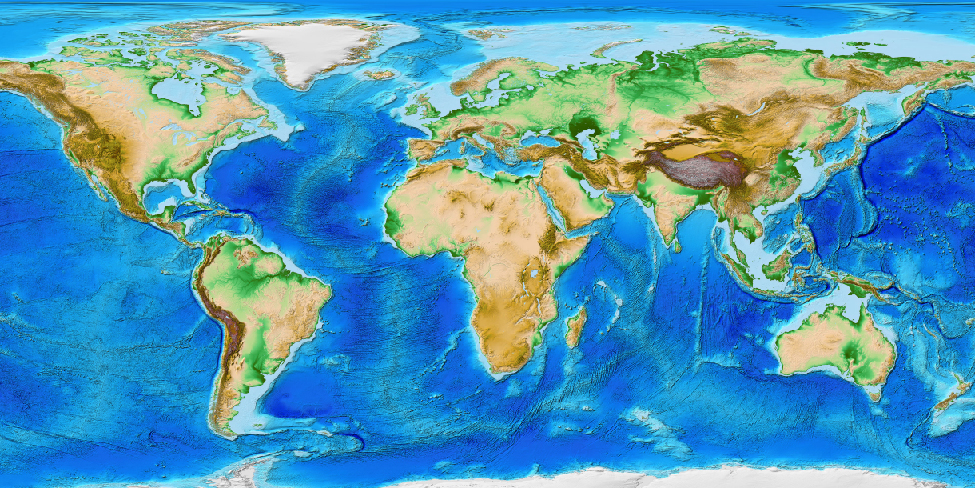
\includegraphics[width=7cm]{Figure8.4}
\end{center}





\clearpage
\subsection*{\ref{uEEpoG} Exercises}

\begin{exercise} \label{qcvlSR}
    What two types of volcanic rock is Earth largely composed of?
\end{exercise}

\begin{exercise}
    List the four layers of Earth's structure, starting from the topmost layer to the innermost.
\end{exercise}

\begin{exercise}
    What percent of the Earth's crust is covered by oceans? 
\end{exercise}

\begin{exercise}
    What percent of the crust is continental (area of land, not ocean)?
\end{exercise}

\begin{exercise}
    How many kilometers thick is ocean crust?
\end{exercise}

\begin{exercise} \label{4pG09w}
    Name the five primary elements found in oceanic crust.
\end{exercise}

\begin{exercise}
    About how many kilometers thick is continental crust?
\end{exercise}


\begin{exercise}
    What percent of Earth's total mass is made up by the crust?
\end{exercise}

\begin{exercise}
    Estimate the thickness of the mantle in miles.
\end{exercise}

\begin{exercise}
    How do scientists analyze the chemistry of the mantle despite the mantle being dozens of miles beneath the ground?
\end{exercise}

\begin{exercise}
    Earth's core is subdivided into two parts: the outer core and the inner core. Which part is solid, and which is liquid?
\end{exercise}

\begin{exercise}
    Name the planet that is smaller in size that Earth's core.
\end{exercise}

\begin{exercise}
    What three substances, compressed to a very high density, are found in the core?
\end{exercise}

\begin{exercise}
    What does Earth's current differentiation (containing layers of different densities) suggest about its early history?
\end{exercise}

\clearpage
\subsection{Magnetic Field and Magnetosphere} \label{17sluw}

We can find additional clues about Earth's interior from its magnetic field. Our planet behaves in some ways as if a giant bar magnet were inside it, aligned approximately with the rotational poles of Earth. This magnetic field is generated by moving material in Earth's liquid metallic core. As the liquid metal inside Earth circulates, it sets up a circulating electric current. When many charged particles are moving together like that---in the laboratory or on the scale of an entire planet---they produce a magnetic field.

\vspace{1em}

Earth's magnetic field extends into surrounding space. When a charged particle encounters a magnetic field in space, it becomes trapped in the magnetic zone. Above Earth's atmosphere, our field is able to trap small quantities of electrons and other atomic particles. This region, called the \gls{magnetosphere}, is defined as the zone within which Earth's magnetic field dominates over the weak interplanetary magnetic field that extends outward from the Sun.

\vspace{1em}


\begin{center}
\begin{tikzpicture}
    \node at (0,0) {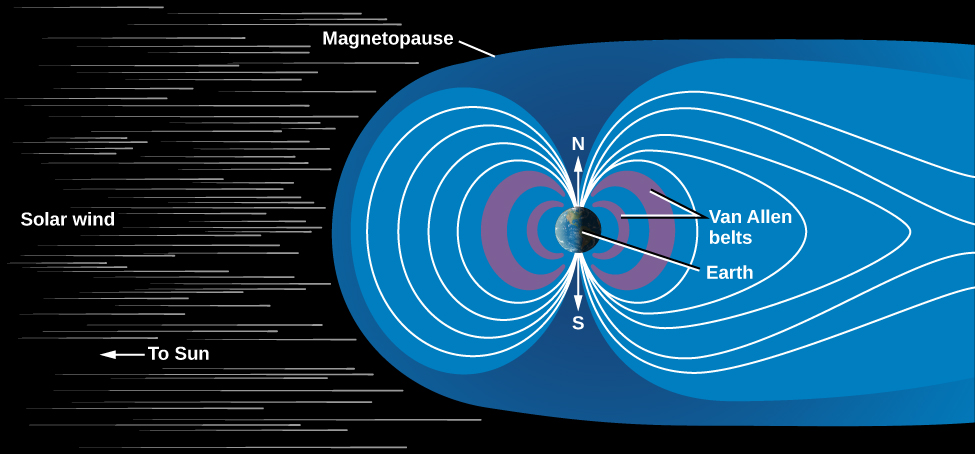
\includegraphics[width=12cm]{Figures/Figure8.5.jpg}};
    \fill[white,opacity=0] (-6,-2.8) rectangle (6,2.8);
    % \draw[red] (-6,-2.8) rectangle (6,2.8);
\end{tikzpicture}
\end{center}

Where do the charged particles trapped in our magnetosphere come from? They flow outward from the hot surface of the Sun; this is called the solar wind. It not only provides particles for Earth's magnetic field to trap, it also stretches our field in the direction pointing away from the Sun. Typically, Earth's magnetosphere extends about 60,000 kilometers, or 10 Earth radii, in the direction of the Sun. But, in the direction away from the Sun, the magnetic field can reach as far as the orbit of the Moon, and sometimes farther.

\vspace{1em}

The magnetosphere was discovered in 1958 by instruments on the first US Earth satellite, Explorer 1, which recorded the ions (charged particles) trapped in its inner part. The regions of high-energy ions in the magnetosphere are often called the Van Allen belts in recognition of the University of Iowa professor who built the scientific instrumentation for Explorer 1. Since 1958, hundreds of spacecraft have explored various regions of the magnetosphere.
\vspace{1ex}
\cyanhrule
\vspace{-1ex}

\begin{multicols}{2}
\subsection*{\ref{17sluw} Exercises}

\begin{exercise}
    Watch ``How Earth's Magnetic Shield Protects Us From The Sun'' (\href{https://youtu.be/URN-XyZD2vQ}{click here}).
\end{exercise}

\begin{exercise}
    \href{https://phet.colorado.edu/en/simulations/magnets-and-electromagnets}{Click here} to access the PhET Simulation ``Magnets and Electromagnets.'' Run the CheerpJ version, and check the box for ``Show planet Earth'' to visualize the directions of Earth's magnetic field lines.
\end{exercise}

\begin{exercise}
    What happens when a charged particle enters a magnetic field?
\end{exercise}

\begin{exercise}
    What generates the Earth's magnetic field?
\end{exercise}

\begin{exercise}
    Earth behaves as if a giant \rule{2cm}{0.15mm} was inside it.
\end{exercise}

\begin{exercise}
    What is the magnetosphere?
\end{exercise}

\begin{exercise}
    What particles does our magnetosphere trap?
\end{exercise}

\begin{exercise}
    Where do the charged particles trapped in our magnetosphere come from?
\end{exercise}

\begin{exercise}
    Earth's magnetosphere was discovered in the year \rule{2cm}{0.15mm}.
\end{exercise}

\begin{exercise}
    What was Professor Van Allen's contribution to the discovery of the magnetosphere?
\end{exercise}
\end{multicols}

\subsection{Structure of the Atmosphere} \label{Qhjd2y}

We live at the bottom of the ocean of air that envelops our planet. The atmosphere, weighing down upon Earth's surface under the force of gravity, exerts a pressure at sea level that scientists define as 1 bar (a term that comes from the same root as barometer, an instrument used to measure atmospheric pressure). A bar of pressure means that each square centimeter of Earth's surface has a weight equivalent to 1.03 kilograms pressing down on it. Humans have evolved to live at this pressure; make the pressure a lot lower or higher and we do not function well.

\vspace{1em}

The total mass of Earth's atmosphere is about \SI{5e18}{} kilograms. This sounds like a large number, but it is only about a millionth of the total mass of Earth. The atmosphere represents a smaller fraction of Earth than the fraction of your mass represented by the hair on your head.

\vspace{1em}

\begin{minipage}{0.5\textwidth}
    The structure of the atmosphere is illustrated in the figure. Most of the atmosphere is concentrated near the surface of Earth, within about the bottom 10 kilometers where clouds form and airplanes fly. Within this region---called the troposphere---warm air, heated by the surface, rises and is replaced by descending currents of cooler air; this is an example of convection. This circulation generates clouds and wind. Within the troposphere, temperature decreases rapidly with increasing elevation to values near \qty{50}{\degreeCelsius} below freezing at its upper boundary, where the stratosphere begins. Most of the stratosphere, which extends to about 50 kilometers above the surface, is cold and free of clouds.
\end{minipage}%
\hspace{10mm}
\begin{minipage}{0.45\textwidth}
    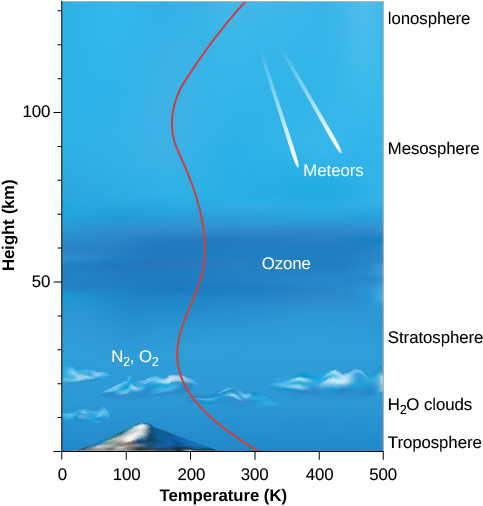
\includegraphics[width=6cm]{Figures/Figure8.12.jpeg}
\end{minipage}

\vspace{1em}

Near the top of the stratosphere is a layer of ozone ($\mathrm{O}_3$), a form of oxygen with three atoms per molecule instead of the usual two. Because ozone is a good absorber of ultraviolet light, it protects the surface from some of the Sun's dangerous ultraviolet radiation, making it possible for life to exist on Earth. The breakup of ozone adds heat to the stratosphere, reversing the decreasing temperature trend in the troposphere. Because ozone is essential to our survival, we reacted with justifiable concern to evidence that became clear in the 1980s that atmospheric ozone was being destroyed by human activities. By international agreement, the production of industrial chemicals that cause ozone depletion, called chlorofluorocarbons, or CFCs, has been phased out. As a result, ozone loss has stopped and the ``ozone hole'' over the Antarctic is shrinking gradually. This is an example of how concerted international action can help maintain the habitability of Earth.

\vspace{1em}

At heights above 100 kilometers, the atmosphere is so thin that orbiting satellites can pass through it with very little friction. Many of the atoms are ionized by the loss of an electron, and this region is often called the ionosphere. At these elevations, individual atoms can occasionally escape completely from the gravitational field of Earth. There is a continuous, slow leaking of atmosphere---especially of lightweight atoms, which move faster than heavy ones. Earth's atmosphere cannot, for example, hold on for long to hydrogen or helium, which escape into space. Earth is not the only planet to experience atmosphere leakage. Atmospheric leakage also created Mars' thin atmosphere. Venus' dry atmosphere evolved because its proximity to the Sun vaporized and dissociated any water, with the component gases lost to space.

\clearpage
\subsection*{\ref{Qhjd2y} Relevant Application: Research Two Atmospheric Layers}
The five layers of the atmosphere, from bottom-most to topmost, are the following:

\begin{enumerate}
    \item troposphere
    \item stratosphere
    \item mesosphere
    \item thermosphere
    \item exosphere
\end{enumerate}

(The ionosphere is not exactly a layer but is rather an area of ionic activity that is spread between the thermosphere and exosphere.) The following exercises will relate to these 5 layers of the atmosphere. Do these exercises on paper.

\begin{exercise}
    Draw a sketch of all five layers. Remember, mountains, clouds, and airplanes are part of the troposphere; the ozone layer, part of the stratosphere; meteors, part of the mesosphere, and so on. You may use \href{https://en.wikipedia.org/wiki/Atmosphere#/media/File:Atmosphere_layers-en.svg}{this image} for inspiration.
\end{exercise}

\begin{exercise} \label{WsEZii}
    You will be assigned 1 layer to research and take notes on. For example, if you are assigned the troposphere, record its thickness and height above the ground, what things it contains, why it has the name it has, etc. Emphasize what makes that layer special. Jot down organized notes in your notebook. We recommend starting at the website \href{https://spaceplace.nasa.gov/atmosphere/en/}{https://spaceplace.nasa.gov/atmosphere/en/} and then searching the web for other reliable sources.
\end{exercise}

\begin{exercise}
    Using the notes taken in the previous exercise, write a brief summary (3 to 5 sentences) of the main ideas about this layer of the atmosphere. Do \textbf{not} copy the website or online source. You must USE YOUR OWN WORDS.
\end{exercise}

\begin{exercise} \label{XqVzFv}
    Create 3 to 5 multiple choice questions about your layer. For example, one of the questions may be:
    \vspace{1em}
    
    \hspace{2em} 1. Which layer contains ozone?
    
    \hspace{3.5em} A. Troposphere
    
    \hspace{3.5em} B. Stratosphere

    \hspace{3.5em} C. Mesosphere

    \hspace{3.5em} D. Thermosphere

    \vspace{1em}

    Finally, create an answer key, so you know which are the correct options.
\end{exercise}

\begin{exercise}
    Pick your \textbf{favorite} multiple choice question you created and copy it on a sticky note, including the choices A, B, C, and D. On the back of the sticky note, write the following four things: the name of the layer, the correct answer choice, your initials, and your Astronomy class period. 
\end{exercise}

\begin{exercise}
    \textit{If time permits}: Pick any other layer you like, and repeat Exercises \ref{WsEZii}--\ref{XqVzFv} for that layer.
\end{exercise}


% \end{multicols}

\clearpage
\subsection*{Answers to Select Exercises}

\ref{qcvlSR}. Basalt and granite\\
\ref{4pG09w}. silicon, oxygen, iron, aluminum, and magnesium\\


\clearpage
\subsection*{Daily Lesson Plans}

\begin{tabular}{|m{0.25\textwidth}|m{0.7\textwidth}|}
    \hline  
    \cellcolor{black!20}\textbf{Date} &
    \cellcolor{black!20}\textbf{Tuesday, February 14, 2023} \\
    \hline
    Learning Intention (TPO) & We will list properties of Earth and share ideas through a whiteboard lecture.\\
    \hline
    Hook/Warm Up/Opening & Take a guess: How far away is the core of our planet?\\
    \hline
    Lesson/Learning Activities & Draw a sketch of Earth. Earth is our home planet and the only known place in the universe with life. List the diameter, rotational period, and distance from the Sun. Fun fact: At 75 mph, in straight line at a constant speed, the time it would take a car to ``drive'' to the Sun is 141 years. List Earth's mass, escape velocity, and surface area. Emphasize that even if you are an avid traveler/explorer, you will only ever touch a TINY fraction of Earth's surface area. Most is unexplored.\\
    \hline
    Graded Activities & Exercises \#\ref{uqgC3z}--\ref{BKbf6Y}\\
    \hline
    Closure & Discuss questions about exercises.\\  
    \hline
\end{tabular}

\begin{tabular}{|m{0.25\textwidth}|m{0.7\textwidth}|}
    \hline  
    \cellcolor{black!20}\textbf{Date} &
    \cellcolor{black!20}\textbf{Tuesday, February 21, 2023} \\
    \hline
    Learning Intention (TPO) & We will... \\
    \hline
    Hook/Warm Up/Opening & \\
    \hline
    Lesson/Learning Activities & Watch \href{https://youtu.be/URN-XyZD2vQ}{this video} on how the Earth's magnetic field protects us. Lecture on the magnetic field and magnetosphere. Ask students to guess what year humans discovered that Earth has a magnetic field. Students write year on sticky note. Create a histogram of years guessed. Offer extra credit to closest answer.\\
    \hline
    Graded Activities & Exercises.\\
    \hline
    Closure & \\  
    \hline
\end{tabular}


\end{document}



\begin{tabular}{|m{0.25\textwidth}|m{0.7\textwidth}|}
    \hline  
    \cellcolor{black!20}\textbf{Date} &
    \cellcolor{black!20}\textbf{***day, Jan, DD 2023} \\
    \hline
    Learning Intention (TPO) & We will []. \\
    \hline
    Hook/Warm Up/Opening & \\
    \hline
    Lesson/Learning Activities & \\
    \hline
    Graded Activities & \\
    \hline
    Closure & \\  
    \hline
\end{tabular}